\documentclass[a4paper,11pt]{article}
\usepackage[spanish]{babel}
\usepackage[utf8]{inputenc}
\usepackage{hyperref}
\usepackage{listings}
\usepackage{mathtools}
\usepackage{graphicx}
\begin{document}
\title{Estudio de la eficiencia del algoritmo de la burbuja en C++}
\author{Noelia Escalera Mejías}
\date{}
\maketitle
\section{Resumen}
URL del repositorio:
\url{https://github.com/Arelaxe/proyecto_final}
\\ \\
Para el proyecto final del curso de LaTeX y Git, he decidido hacer un estudio sobre la eficiencia del algoritmo de la burbuja, de forma tanto teórica como empírica.
\section{Palabras clave}
\begin{itemize}
\item {\bf Algoritmo:} Conjunto finito de pasos que nos llevan a resolver un problema.
\item {\bf Implementación:} Realización de un algoritmo en un lenguaje de programción determinado.
\item {\bf Eficiencia:} Capacidad de lograr resolver un algoritmo con el mínimo de recursos posibles o en el menor tiempo posible.
\item {\bf C++:} Lenguaje de programación diseñado en 1979 por Bjarne Stroupstrup, con la intención de extender al lenguaje de programación C mecanismos que permiten la manipulación de objetos.
\item {\bf Bash:} Programa informático, cuya función consiste en interpretar órdenes, y un lenguaje de consola.
\item {\bf Gnuplot:} Programa para generar gráficas de funciones y datos.
\item {\bf Algoritmo de la Burbuja \it (Bubble Sort):} Sencillo algoritmo de ordenación. Funciona revisando cada elemento de la lista que va a ser ordenada con el siguiente, intercambiándolos de posición si están en el orden equivocado.
\end{itemize}
\section{Introducción}
El algoritmo de la burbuja es uno de los primeros algoritmos de ordenación que se aprenden a programar debido a la sencillez de su implementación. Sin embargo, ¿es eficiente? Esto es lo que vamos a comprobar en el presente informe. El lenguaje de programación en el que se trabajará será C++11.
\section{Estado del arte}
La eficiencia teórica del algoritmo de la burbuja está ya bastante estudiada, debido a que es un algoritmo bastante conocido. Para estudiarla hemos usado las principales reglas para medir la eficiencia de bucles: sumatorios y reglas de progresiones aritméticas, así como la notación O.
\section{Eficiencia teórica}
Hay varias formas de implementar el algoritmo de la burbuja. Nosotros usaremos la más sencilla:
\lstset{language=C, breaklines=true, basicstyle=\footnotesize}
\begin{lstlisting}[frame=single]
void ordenar(int *v, int n) {
 for (int i=0; i<n-1; i++)
  for (int j=0; j<n-i-1; j++)
   if (v[j]>v[j+1]) {
    int aux = v[j];
    v[j] = v[j+1];
    v[j+1] = aux;
   }
}
\end{lstlisting}
La eficiencia teórica sería la siguiente:\\ \\
\begin{large}
{\bf -Bucle for: Se ejecuta n-1 veces}
\end{large}
\begin{itemize}
\item {\bf Línea 2:} 4 operaciones, Asignación $(i=0)$, Resta $(n-1)$, Comparación $(i<n-1)$ e Incremento $(i++)$. 3 operaciones se ejecutan a la vez y otras tres se ejecutan n veces.
\end{itemize}
\begin{large}
{\bf -Bucle for (dentro del for anterior: Se ejecuta n-i-1 veces, es una progresión aritmética)}
\end{large}
\begin{itemize}
\item {\bf Línea 3:} 5 operaciones. Asignación $(j=0)$, Resta $(n-i,(n-i)-1)$, Comparación $(j<n-i-1)$ e Incremento $(j++)$. 4 operaciones se ejecutan una vez y otras 4 se ejecutan n veces.
\end{itemize}
\begin{large}
{\bf -If (dentro del for anterior): Se ejecuta siempre, ya que estamos en el peor de los casos}
\end{large}
\begin{itemize}
\item {\bf Línea 4:} 4 operaciones, Acceso a vectores $(v[j],v[j+1])$, Suma $(j+1)$, Comparación $(v[j]>v[j+1])$.
\item {\bf Línea 5:} 2 operaciones, Acceso a vector $(v[j])$, Asignación $(aux=v[j])$.
\item {\bf Línea 6:} 4 operaciones, Acceso a vectores $(v[j],v[j+1])$, Asignación $(v[j]=v[j+1])$, Suma $(j+1)$.
\item {\bf Línea 7:} 3 operaciones, Acceso a vector $(v[j+1])$, Suma $(j+1)$, Asignación $(v[j+1]=aux)$. 
\end{itemize}
Por tanto, el tiempo en el peor de los casos sería: 
\begin{displaymath}
3+\sum_{i=0}^{n+1}(3+4+\sum_{j=0}^{n-i-1}(4+4+2+4+3))=3+3+\sum_{i=0}^{n-1}(7+17(n-i-1))=
\end{displaymath}
\begin{displaymath}
=3+(n-1)\frac{7+17(n-n+3-1)+7+17(n+1)}{2}=3+(n+1)\frac{7+17+2+7+17n+17}{2}=
\end{displaymath}
\begin{displaymath}
=3+(n-1)\frac{17n+65}{2}=3+\frac{17n^2+65n-17n-65}{2}=\frac{17n^2+48n-59}{2}
\end{displaymath}
Luego podemos decir que tenemos una eficiencia de $O(n^2)$.
\section{Eficiencia empírica}
Para calcular la eficiencia empírica hemos usado los siguientes ficheros fuente:
\lstset{language=C, breaklines=true, basicstyle=\footnotesize}
\begin{lstlisting}[frame=single]
#include <iostream>
#include <ctime> // Recursos para medir tiempos
#include <cstdlib> // Para generacion de  numeros pseudoaleatorios

using namespace std;

void ordenar(int *v, int n) {
 for (int i=0; i<n-1; i++)
  for (int j=0; j<n-i-1; j++)
   if (v[j]>v[j+1]) {
    int aux = v[j];
    v[j] = v[j+1];
    v[j+1] = aux;
   }
}

void sintaxis()
{
 cerr << "Sintaxis:" << endl;
 cerr << " TAM: Tam del vector (>0)" << endl;
 cerr << " VMAX: Valor max (>0)" << endl;
 cerr << "Se genera un vector de tam TAM con elementos aleatorios en [0,VMAX[" << endl;
 exit(EXIT_FAILURE);
}

int main(int argc, char * argv[])
{
 // Lectura de parametros
 if (argc!=3)
  sintaxis();
 int tam=atoi(argv[1]); // Tam del vector
 int vmax=atoi(argv[2]); // Valor max
 if (tam<=0 || vmax<=0)
  sintaxis();
  
 // Generacion del vector aleatorio
 int *v=new int[tam]; // Reserva de memoria
 srand(time(0)); // Inicializacion del generador de nums pseudoaleatorios
 for (int i=0; i<tam; i++) // Recorrer   vector
  v[i] = rand() % vmax; // Generar aleatorio [0,vmax[
 clock_t tini; // Anotamos el tiempo de inicio
 tini=clock();
 int x = vmax+1;
 ordenar(v,tam);
 clock_t tfin; // Anotamos el tiempo de finalizacion
 tfin=clock();
 // Mostramos resultados
 cout << tam << "\t" << (tfin-tini)/(double)CLOCKS_PER_SEC << endl;
 delete [] v; // Liberamos memoria dinamica
}
\end{lstlisting}
\lstset{language=Bash, breaklines=true, basicstyle=\footnotesize}
\begin{lstlisting}[frame=single]
#!/bin/csh
@ inicio = 100
@ fin = 30000
@ incremento = 100
set ejecutable = ordenacion
set salida = tiempos_ordenacion.dat
@ i = $inicio
echo > $salida
while ( $i <= $fin )
echo Ejecucion tam = $i
echo `./{$ejecutable} $i 10000` >> $salida
@ i += $incremento
end
\end{lstlisting}
Hemos compilado el programa ordenacion.cpp de la siguiente manera:
\begin{center}
{\bf \it g++ ordenacion.cpp -o ordenacion}
\end{center}
Tras ejecutar el script ejecucuiones\_ordenacion.csh: 
\begin{center}
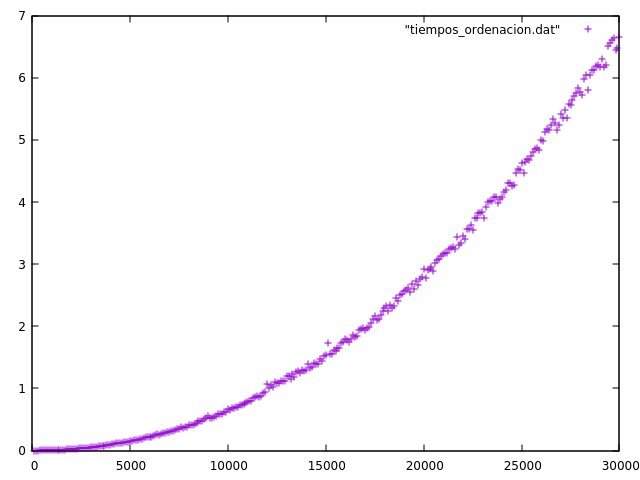
\includegraphics[scale=0.5]{1}
\end{center}
A continuación, vamos a obtener el ajuste de regresión para el algoritmo anterior. Para realizar este ajuste, supondremos que $f(x)=ax^2+bx+c$ es la función a la que queremos ajustar nuestros tiempos. Según gnuplot, los valores más adecuados para a, b y c son:
\begin{center}
{\it a=8.11499e-09 \\ b=-1.26893e-05 \\ c=0.0486703}
\end{center}
Si dibujamos superpuestas f(x) y la función tiempos\_ordenacion.dat, nos queda lo siguiente:
\begin{center}
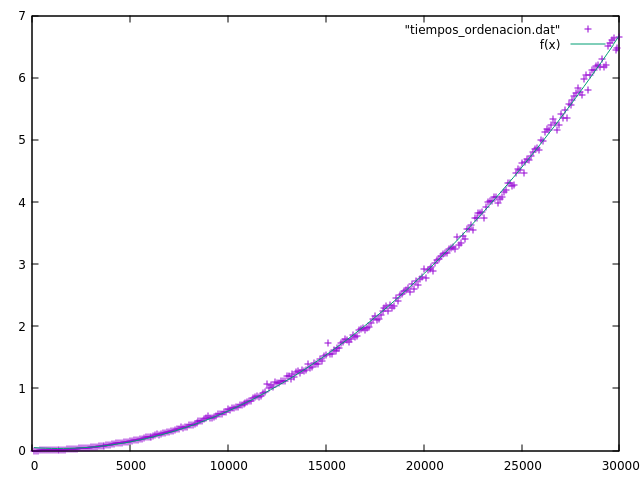
\includegraphics[scale=0.5]{2}
\end{center}
\bibliography{bibliografia}
\bibliographystyle{plain}
\nocite{*}
\end{document}